The first step we need to take is analyzing the effect of varying a trajectory first. In general, one can expect to vary the trajectory followed by the system in two ways: given a control, varying the initial conditions or, given the initial conditions, varying the control. Nevertheless it is still necessary to develop some tools to \textit{describe} the variation of a trajectory. 

\subsection{Variations and adjoint response}


\paragraph{Variational and adjoint equations}\mbox{}\\
Given a control system \controlSystem\space and an admissible u $\mu:I\fd U$ we define the following:
\lista{
	\item the \grass{variational equation}  equation for $\Sigma$ with control $\mu$ is the differential equation
	\begin{multiLineSingleNumber}
		\statotdot=f(\statot,\mut);\\
		\dot{v}(t)=\Dderarg{1}f(\statot,\mut)\cdot v(t)\\
		(\statot,\mut)\in(\chi\times\R^n)
		\label{variational-equation}
	\end{multiLineSingleNumber}	
	
	
	\item the \grass{adjoint equation}  equation for $\Sigma$ with control $\mu$ is the differential equation
	\begin{multiLineSingleNumber}
		\statotdot=f(\statot,\mut);\\
		\lambdatdot=-\Dderarg{1}f^T(\statot,\mut)\cdot v(t)\\
		(\statot,\lambdat)\in(\chi\times\R^n)
		\label{adjoint-equation}
	\end{multiLineSingleNumber}
ù}

\subparagraph{Interpretation}It is straightforward to see that the variational equation describes, through a linearization,  the evolution in time of a small (infinitesimal) variation from the original trajectory $\statot$, solution to \eqref{e1.1}.\\
Obviously, we hope that given a certain control and initial condition, the solution to \eqref{e1.1} is unique, but a-priori it cannot be said.\\
The geometrical interpretation of the adjoint equation is more subtle, but, in a naive way, one could say that, given an optimal trajectory, the adjoint response is a vector orthogonal to the hyerplane given by (the directions of ) the possible (infinitesimal) variations to that trajectory. 



\subsection{Variations and infinitesimal variations}

\paragraph{Definitions}\mbox{}\\
Let \controlSystem\space be a control system, $x_0\in\chi$ be an initial condition for eq. \eqref{e1.1}, $\tzto\subset\R$ a time interval, $\mu\in\admContr{x_0,t_0,\tzto}$. A \grass{variation} of the trajectory \trajWinCond{\cdot} is a map $\sigma:J\times\tzto\fd\chi$ with the following properties: 
\lista{
	\item $J\subset\R;0\in int(J)$,
	\item $\sigma(0,t)=$\trajWinCond{t} for each $t\in\tzto$,
	\item $s\fd\sigma(s,t)\text{is of class }C^1\text{ for each }t\in\tzto$,
	\item $t\fd\sigma(s,t)$ is a solution of eq. \eqref{e1.1}.
}

Given a variation and its relative trajectory, there is another important quantity, which is he corresponding \grass{infinitesimal variation}. This is yet another map defined with the following limit
\equaz{
	\delta\sigma(t)=\frac{d}{ds}\bigg\rvert _{s=0}\sigma(s,t).
	\label{infinitesimal-variation-definition}
}
\begin{figure}[H]
	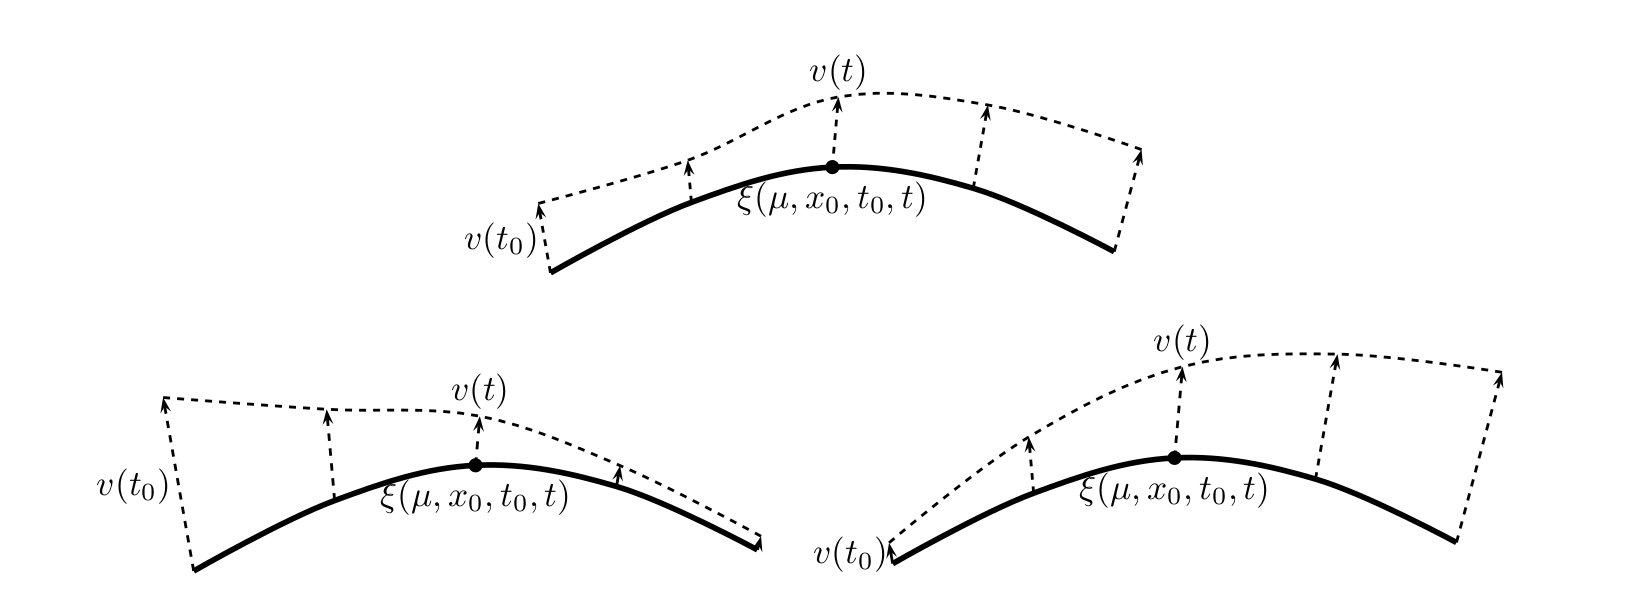
\includegraphics[width=\linewidth]{imgs/variations.png}
	\caption{The dotted arrow represent the difference between the variation (at various times and at a given s), and the "original" trajectory, at the same time. The infinitesimal variation is then represented by a vector such that, at a given time $\overline{t},\space\sigma(s,\overline{t})\approx$\trajWinCond{\overline{t}}$+s\delta\sigma(\overline{t})$
		Actually, there is another interpretation to the image, in which the dotted arrow are the vectors represent the \grass{infinitesimal} variations, and the dotted line is just the envelope of the dotted arrows calculated at different times. In this case, the dotted part and the continuous-line of the figure have scales that have nothing to do one with each other. Nevertheless, in both interpretations, it is possible to understand the concept of a stable, unstable and "indifferent" trajectory, in which a disturbance in the trajectory is amplified rather than muted.}
	\label{fig-variations}
\end{figure}


\paragraph{A theorem about infinitesimal variations}Here it will be stated that if a map is solution of equation \eqref{variational-equation} then it is an infinitesimal variation, and vice versa.\\
Let \controlSystem\space be a control system, $x_0\in\chi$ be an initial condition for eq. \eqref{e1.1}, $\tzto\subset\R$ a time interval, $\mu\in\admContr{x_0,t_0,\tzto}$. Given a map $v:\tzto\fd\R^n$ the statements \lista{
	\item there exists a map $\sigma$ which is a variation of \trajWinCond{\cdot} such that $v=\delta\sigma$ and
	\item $t\fd($\trajWinCond{t}$,v(t))$ satisfies the variational equation \ref{variational-equation}
}
are equivalent. 

\subparagraph{The foundamental matrix $\Phi$}We temporarily define an $n\times n$ linear map $\Phi(t):\R^n\fd\R^n$ as a map such that $\Phi(t)\cdot w=\Dderarg{2}$\trajWinCond{t}$\cdot w$.\\
By differentiation one can see that $\Phi(t)$ satisfies this matrix differential initial value problem
\begin{gather*}
\dot{\Phi}(t)=\Dderarg{1}f(\trajWinCondMath{t},\mut)\circ\Phi(t);\text{   	   }\Phi(t_0)=Id_{n\times n}.
\end{gather*}

We can re-define, for wider generality, $\fondMatMath{\tau}{t}$ by the solution to the matrix initial value problem 
\begin{equation*}
	\dot{\Phi}(t)=\Dderarg{1}f(\trajWinCondMath{t},\mut)\circ\Phi(t);\text{   	   }\Phi(\tau)=Id_{n\times n},
\end{equation*}
where of course $t,\tau\in\tzto$.\\

The importance of this matrix resides in the fact that, being the variational equation \eqref{variational-equation} a linear one and being $\Phi$ the fundamental matrix of the equation, it is true that, for a variation $v(t)$ (which is also a solution to the variational equation), $v(t)=\fondMatMath{t_0}{t}\cdot v(t_0)$.\\


\subsection{Properties of adjoint repsonse }
What this theorem says is that seeing \eqref{adjoint-equation} and \eqref{adjoint-hamiltonian} are equivalent.

\paragraph[prop 4.4]{Hamilton's and adjoint equation}\mbox{}\\
\grass{Theorem}: given a control system \controlSystem, an admissible control $\mu:I\fd U$, and two maps $\xi:I\fd\chi;$\space$\lambda:I\fd\R^n$, those two statements are equivalent: \lista{
	\item the curve $t\fd(\statot,\lambdat)$ satisfies the adjoint equation \eqref{adjoint-equation},
	\item the curve $t\fd(\statot,\lambdat)$ satisfies the differential equation \eqref{adjoint-hamiltonian} recalled here:
		\begin{gather*}
				\statotdot=D_2H_\Sigma(\statot,\lambdat,\mut)\\
				\lambdat=-D_1H_\Sigma(\statot,\lambdat,\mut)
		\end{gather*}
}
This theorem is demonstrated simply by differentiating the given quantities, and by using the properties of dot product. 


\paragraph[prop 4.5]{Adjoint response and variations}\mbox{}\\
\grass{Theorem:} Let \controlSystem\space be a control system, $x_0\in\chi$ be an initial condition for eq. \eqref{e1.1}, $\tzto\subset\R$ a time interval, $\mu\in\admContr{x_0,t_0,\tzto}$. If $v$ and $\lambda$ are two maps $v,\lambda:\tzto\fd\R^n$ that satisfy the variational and adjoint equation respectively (toghether with the trajectory $t\fd$\trajWinCond{t}), then 
\begin{equation*}
	\langle\lambdat,v(t)\rangle=\langle\lambda(t_0),v(t_0)\rangle
\end{equation*}
for all $t\in\tzto$.\\
\grass{Proof:}
\begin{gather*}
	\frac{d}{dt}\langle\lambdat,v(t)\rangle=\\
	\langle\lambdatdot,v(t)\rangle+	\langle\lambdat,\dot{v}(t)\rangle=\\
	-\langle\Dderarg{1}f^T(\controlledTrajMath)\cdot\lambdat,v(t)\rangle +\langle\lambdat,\Dderarg{1}f^T(\controlledTrajMath)\cdot v(t)\rangle=0.
\end{gather*}

\subparagraph[4.6]{A corollary}An important consequence of this fact is that if the two vectors $v,\lambda$ are orthogonal at the initial moment, they remain orthogonal throughout the whole evolution of the system. 


\paragraph[prop 4.7]{Foundamental matrix for the adjoint response.}\mbox{}\\
\grass{Theorem:} Let \controlSystem\space be a control system, $x_0\in\chi$ be an initial condition for eq. \eqref{e1.1}, $\tzto\subset\R$ a time interval, $\mu\in\admContr{x_0,t_0,\tzto}$, and let $\tau\in\tzto$. Then the solution of the initial value problem 
\gatherNo{\lambdatdot=-\Dderarg{1}f^T(\statot,\mut)\cdot v(t),\text{      	}\lambda(\tau)=\lambda_\tau }
is the following one:
\gatherNo{t\fd\lambdat=\fondMatMath{t}{\tau}^T\cdot\lambda_\tau  }